\chapter{Stability \& Control}
\setlength{\parindent}{15pt}
\label{ch:stab_cont}

\section{Design Approach}

Different design options can be considered in order to control the UAV and ensure stability of the UAV. In the concept selection phase, the decision has been made to have a tail for stability and control surfaces for control in horizontal flight whereas propellers are used for control and stability in vertical flight. First of all, the tail was sized for longitudinal and lateral control and stability considering the critical case of one engine failure. A tail configuration was selected based on effectiveness and controllability. The required surface area of the vertical and horizontal tail were calculated and the optimal incidence angle of the horizontal tail was found. Simultaneously, the c.g. range needed to be estimated and controlled using the position of the wing as a balancing tool. Next, the control surfaces and actuators were sized in order to provide the required angular acceleration. Thereafter, the propeller power split in order to perform manoeuvres during vertical flight was calculated. Finally, the transition phase was considered and a series of actions was defined in order to have a smooth transition. \autoref{fig:StabContFlow} shows the work flow diagram for the stability and control design process. %this is an overview of the work flow

The design process of the tail is an iterative process where mainly the global c.g. position changes. In order to know the global c.g. the tail needs to be sized. Vice versa, in order to size the tail, the c.g. needs to be known. By using the mass budget and an initial placement of the subsystems, an initial c.g. estimation was made. This estimation was used as a starting point for the tail sizing and wing positioning. Eventually, a more updated c.g. was found using CATIA so the design could be iterated. %this is some more explanation on the tail iteration

Also the design process of the control principle is an iterative process. Similar to the c.g., the Moment Of Inertia (MOI) changes throughout the design phase. Again, an initial estimation of the MOI was made in order to estimate the required control moments. Next, in order to size the control surfaces, the arm needed to be known which depend on the size of the control surface. Therefore, another iteration process was needed. %here will be some more explanation on the control surface iteration

\nomenclature[A]{MOI}{Moment Of Inertia}

\begin{figure}[htb]
    \centering
    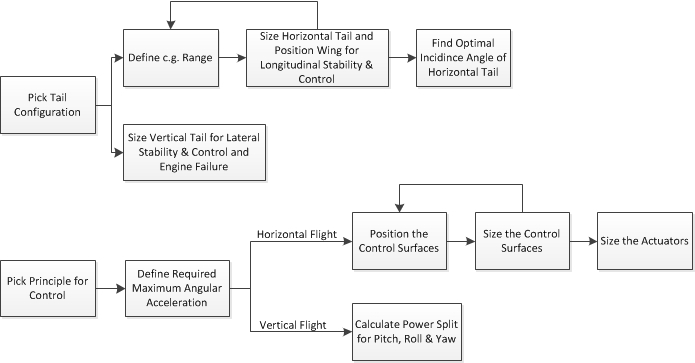
\includegraphics[width=\textwidth]{StabilityandControl/Figures/ApproachFlow2}
    \caption{Work Flow Diagram for the Stability \& Control Design Process}
    \label{fig:StabContFlow}
\end{figure}

\section{Assumptions}

\begin{itemize}
    \item It is assumed that the c.g. coincides with the a.c. of the wing. Since the c.g. is located at ... m from the nose and the a.c. of the wing is located at ... m from the nose, this assumption can be used in the design process without heavily affecting the final results.
    \item It is assumed that the C$_L$ of the horizontal tail during stall with elevator fully deflected is equal to -0.8. This value is derived from statistical data for aircraft with adjustable tails \cite{SEAD}.
    \item It is assumed that the resultant force of a control surface goes through half the chord of the control surface. Conventionally, the resulting force is taken through a quarter chord. However, the flow over the control surface is heavily affected by the airfoil in front of it. By putting the resultant force through half the chord, the arm of the force to the hinge is slightly larger than the actual arm. Therefore, The actuators will be slightly over-designed.
    \item add assumption for the payload bay.
    \item add assumptions for vertical tail sizing.
    %Gervase - Add some assumptions for vertical tail sizing
\end{itemize}

\section{Analysis}

\subsection{Horizontal Flight Phase}



\paragraph{Longitudinal Stability \& Control}



\begin{figure}[htb]
    \centering
    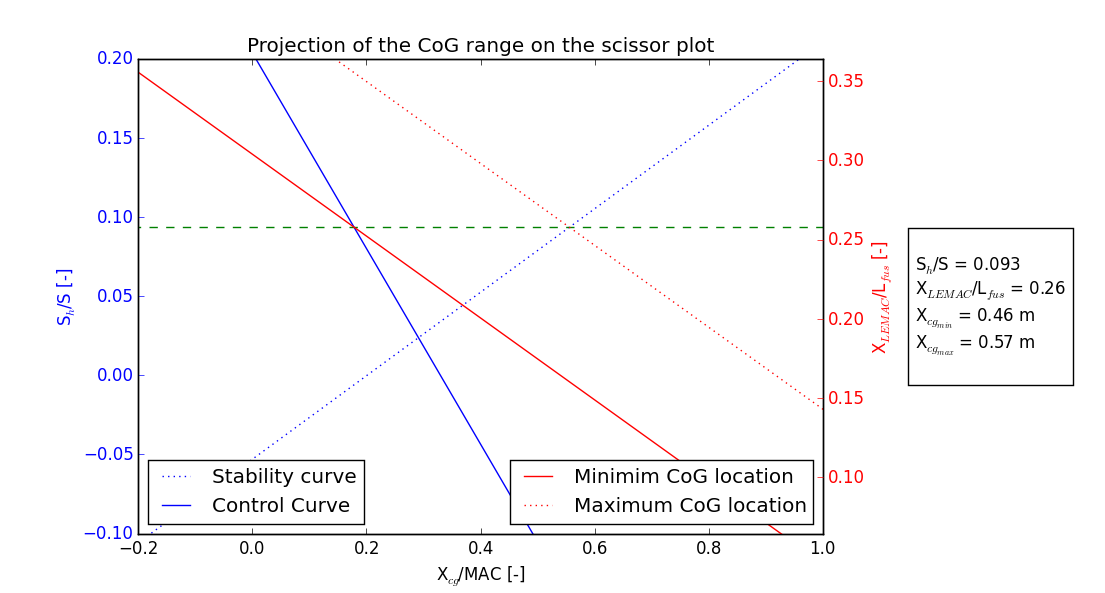
\includegraphics[width=\textwidth]{StabilityandControl/Figures/ScissorVScg3}
    \caption{Projection of the c.g. range on the scissor plot}
    \label{fig:scissor}
\end{figure}

\paragraph{Lateral Stability \& Control}

\paragraph{Control Surfaces}

In this section, the size and position of the control surfaces is determined. These are ailerons for roll control, an elevator for pitch control and a rudder for yaw control. Then, the hinge moment is calculated in order to obtain suitable servos. 

The design of the control surfaces is mainly dependant on the angular accelerations required. After some literature study, the following angular accelerations have been defined for the design of the control surfaces: 
\begin{equation*}
    \alpha_{roll} = \alpha_{pitch} = 45 \frac{^\circ}{s^2} \quad \alpha_{yaw} = 6 \frac{^\circ}{s^2}
\end{equation*}
Then, using the moments of inertia, the torque required is obtained using \autoref{eq:newton2}.
\nomenclature[G]{$\alpha_{roll}$}{Angular roll acceleration}
\nomenclature[G]{$\alpha_{pitch}$}{Angular pitching acceleration}
\nomenclature[G]{$\alpha_{yaw}$}{Angular yaw acceleration}
\begin{equation}
    T = I \cdot \alpha
    \label{eq:newton2}
\end{equation}
These torques have to be created by the control surfaces and hence depend strongly on the physical location of the control surfaces. The elevator is located at the trailing edge of the horizontal tailplane. The moment arm created by that force is set equal to the distance between the center of gravity and the center of the horizontal tailplane. The ailerons are positioned as far away from the fuselage as possible in order to maximise the moment arm. In order to avoid twisting the control surfaces themselves, they can not be positioned at the wing tips themselves. For this reason, they will be positioned just before the start of the wing twist.[DO YOU UNDERSTAND WHAT I MEAN BY THIS?] Then, the rudder is located at the leading edge of the vertical tailplane. The moment arm of the force it creates is the distance between center of gravity and center of the vertical tail. 

Having established necessary torques and moment arms, it is now possible to calculate the required force for the surface itself. The force generated by extracting the surfaces to an angle $\delta$ is given by \autoref{eq:cont_forc}.

\begin{equation}
    F = C_{n_{\delta}}\cdot \delta\cdot\frac{1}{2}\cdot\rho\cdot V^2 \cdot S
    \label{eq:cont_forc}
\end{equation}

In \autoref{eq:cont_forc}, $C_{n_{\delta}}$ is obtained using an xflr analysis.. Then, in order to size the control surfaces, they are designed for stall speed. This ensures that the surface is capable of providing enough force for the whole speed range. Comparing control surface deflection angles of different aircraft, the following maximum deflection angles were defined: 
\nomenclature[B]{$C_{n_{\delta}}$}{Normal Force Gradient}
\nomenclature[G]{$\delta$}{Control surface deflection angle}
\begin{equation*}
    \delta_{elevator_{max}} = 28^\circ\quad\delta_{rudder_{max}} = 25^\circ\quad\delta_{aileron_{max}} = 30 ^\circ
\end{equation*}
Using these parameters, it is now possible to calculate the surface area of the different control surfaces by rearranging \autoref{eq:cont_forc}. 
Then assuming aileron chord to be 20\% of the wing chord, elevator span to be 70\% of the horizontal tailplane span and rudder span to be 90\% of the vertical tailplane span, chord, span and surface area are obtained. The final values are illustrated in \autoref{tab:cont_surf}. The values given for the ailerons are the properties for the aileron on one side of the wing. 

\begin{table}[htb]
    \centering
    \begin{tabular}{lccc}
      \toprule
        & Span [cm]& Chord [cm]& Surface Area [$cm^2$]\\
      \midrule
      Aileron & 17.1 & 3.69 & 63.1 \\\hdashline
      Elevator & 47.2 &2.89& 136 \\\hdashline
      Rudder & 16.3 & 2.67 & 43.4\\\bottomrule
    \end{tabular}
    \caption{Control Surface Dimensions}
    \label{tab:cont_surf}
\end{table}

Using the dimensions of the different control surfaces, an appropriate servo has now to be chosen. For this, it is necessary the calculate the torque required to maintain a certain deflection. 

\begin{figure}[htb]
    \centering
    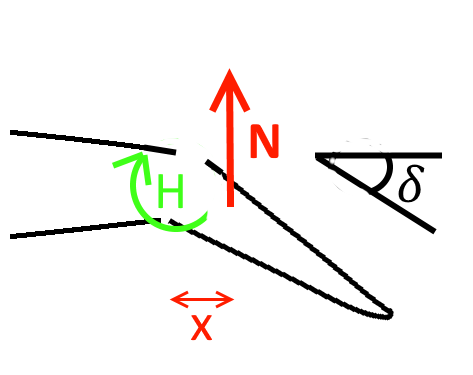
\includegraphics[scale=1]{./StabilityandControl/Figures/hinge}
    \caption{Hinge moment created by the control surface force}
    \label{fig:hing}
\end{figure}

As can be seen in \autoref{fig:hing}, the hinge moment created by the normal force N is dependant on the aerodynamic center of the 

\subsection{Vertical Flight Phase} %This is subject to change

During the vertical flight phase of the the UAV various manoeuvres have to be considered, namely pitch, roll and yaw, all of which are achieved purely through varying the thrust level of the four propellers. By varying the power applied to motor couples the required moments about the axis around which the manoeuvre takes place can be produced. In this section the power required to achieve specified angular accelerations about the three axes will be characterised. However it is necessary to first define the locations of the four motors with respect to the centre of gravity.

\paragraph{General Layout of Motors}
As explained in \autoref{ch:powe_prop} the four motor-propeller combination was chosen to provide most of the thrust during the vertical flight phase whereas the aft motor-propeller combination was chosen to propel the UAV during horizontal flight. For this very reason, during vertical flight, the front propellers are providing most of the thrust.  This results in the distance from the centre of gravity to the fore motors being smaller than the distance from the centre of gravity to the aft motors in the longitudinal direction. For control reasons and simplicity's sake it is beneficial if the lateral and longitudinal distances between the motors are equal. 
It was also import to define the direction of rotation of the moto

\subsection{Transition}
%Finally, the transition phase was considered and a series of actions was defined in order to have a smooth transition.

\section{Verification \& Validation}

\section{Results}
